\documentclass{article}

% Using template from: https://www.overleaf.com/latex/templates/neurips-2023/vstgtvjwgdng

% if you need to pass options to natbib, use, e.g.:
%     \PassOptionsToPackage{numbers, compress}{natbib}
% before loading neurips_2023


% ready for submission
% \usepackage{neurips_2023}


% to compile a preprint version, e.g., for submission to arXiv, add add the
% [preprint] option:
% \usepackage[preprint]{neurips_2023}


% to compile a camera-ready version, add the [final] option, e.g.:
\usepackage[final]{neurips_2023}


% to avoid loading the natbib package, add option nonatbib:
%    \usepackage[nonatbib]{neurips_2023}


\usepackage[utf8]{inputenc} % allow utf-8 input
\usepackage[T1]{fontenc}    % use 8-bit T1 fonts
\usepackage{hyperref}       % hyperlinks
\usepackage{url}            % simple URL typesetting
\usepackage{booktabs}       % professional-quality tables
\usepackage{amsfonts}       % blackboard math symbols
\usepackage{nicefrac}       % compact symbols for 1/2, etc.
\usepackage{microtype}      % microtypography
\usepackage{xcolor}         % colors
\usepackage{graphicx}
\usepackage{bm}
\usepackage{caption}

\graphicspath{ {./images/} }


\title{Quantifying a Global Measure of Credibility Using the Simplex Method}


% The \author macro works with any number of authors. There are two commands
% used to separate the names and addresses of multiple authors: \And and \AND.
%
% Using \And between authors leaves it to LaTeX to determine where to break the
% lines. Using \AND forces a line break at that point. So, if LaTeX puts 3 of 4
% authors names on the first line, and the last on the second line, try using
% \AND instead of \And before the third author name.


\author{%
  Gurpreet Johl \\
  DPhil Applicant \\
  \href{mailto:gurpreetjohl@gmail.com}{\texttt{gurpreetjohl@gmail.com}}
  % examples of more authors
  % \And
  % Coauthor \\
  % Affiliation \\
  % Address \\
  % \texttt{email} \\
  % \AND
  % Coauthor \\
  % Affiliation \\
  % Address \\
  % \texttt{email} \\
  % \And
  % Coauthor \\
  % Affiliation \\
  % Address \\
  % \texttt{email} \\
  % \And
  % Coauthor \\
  % Affiliation \\
  % Address \\
  % \texttt{email} \\
}


\begin{document}


\maketitle

\begin{abstract}
Understanding when a model is appropriate for a given data set is a key consideration when deploying ML models in practice, but this is not straightforward.
Accuracy on a test data set is often used for this purpose, but this does not take into account the confidence in those predictions; a model may be extrapolating far beyond the bounds of its training set and still achieve reasonable accuracy.
This is especially true when data sets are limited in size---by testing multiple models one may find a model with high test accuracy by luck.
Simplex provides a method to explain a given test example in terms of a corpus of examples. This paper extends the Simplex approach to provide a single global value that answers the question "How much the model needed to extrapolate in order to arrive at these outputs for this data set?"
which can serve as a measure of confidence in the model for the given setting.
If a model achieves good accuracy but with a high degree of extrapolation, we may want to be wary of this when using the results in practice.
This gives practitioners another perspective of the applicability of a model for their data set.
This paper proposes possible formulations of such a distance measure and illustrates the use case in a medical application.
\end{abstract}



\section{Introduction}

A key consideration when applying machine learning models in real-world settings is model evaluation---how do we choose the best model and how confident can we be in its outputs? This is an open question, with practitioners relying on heuristics and judgement based on a number of accuracy and confidence measures\cite{ding_model_2018}\cite{raschka_model_2020}.
This is particularly relevant in settings such as healthcare because data is often limited and the impact of decisions based on these models is significant. Having a better understanding of the applicability of a model for a given task, including its strengths and limitations, can help to reduce negative outcomes caused by spurious predictions and biases against groups underrepresented in the training data, thus improving health inequality.

The Simplex approach \cite{crabbe_explaining_2021} can be used to explain individual predictions of a particular model in terms of either examples or features. A particular application of this explored in the original paper is to identify examples from a different distribution using the residuals of the latent approximation, in effect measuring the degree of extrapolation required by the model in order to classify a particular instance.

This research aims to extend this method by aggregating this concept over the test data set, to provide a global quantification of the degree of extrapolation. For a given data set, to what extent does a particular model need to extrapolate beyond the data it was trained on? Intuitively, we may want to be more sceptical of models with a high degree of extrapolation, so this effectively provides a measure of confidence. This scenario is investigated with a real-world application in Section \ref{sec:cancer results}---given a cancer detection image classification model which, unbeknownst to us, has only been trained on images of lungs, can we identify when the model is operating outside of its circle of competence? This can guide practitioners in cases where extra caution should be exercised when following the model's outputs, even when the accuracy is high.

This has implications in model selection, transfer learning and data-centric AI among others. The benefit of such a confidence measure is that the same Simplex methodology can be used as an end-to-end solution for identifying and addressing issues with data and models---the global confidence measure can be used to identify suboptimal model-data combinations, and this can then be understood in terms of both features and examples in order to rectify any issues.


\paragraph{Related works}

The concept of latent space distances as a measure of interpretability is used in the Deep k-Nearest approach \cite{papernot_deep_2018} and this is applied in the context of confidence and credibility. Confidence is defined as "how likely the prediction is to be correct according to the model’s training set", while credibility quantifies "how relevant the training set is to make this prediction". The distance measures presented hereafter provide a measure of extrapolation which may therefore fit the definition of credibility more closely than confidence, although these are closely coupled. Distinguishing between confidence or credibility is not the focus of this work, so these terms will be used interchangeably hereafter. The importance of an extrapolation measure was noted in the context of the Deep KNN approach: “When one wishes to deploy ML in settings where safety or security are critical, it becomes necessary to invent mechanisms suitable to identify when the model is extrapolating too much from the representations it has built with its training data.”

The idea of a single scalar value encapsulating the interpretability of a model is discussed as a desired attribute in the context of \textit{Concept Activation Vectors} \cite{kim_interpretability_2018}, where "plug-in readiness" and "global quantification" are explicit goals of the research. A measure based on the Simplex residuals has the former, by virtue of being a post-hoc explainability technique. This work focuses on extending Simplex to provide a "global quantification" measure of confidence.

Various evaluation measures are discussed by Ding et al. \cite{ding_model_2018} While these primarily focus on the model's performance on a given task rather than interpretability or confidence, we later discuss possible avenues of future research that more closely align accuracy and confidence measures, as illustrated in Figure \ref{explainability_loop}.
The relative importance assigned to performance and confidence measures when selecting between models is subjective. Rechkemmer and Yin observed that respondents claimed to base decisions on confidence but in fact follow the model with the highest accuracy, suggesting that model selection choices are often based on accuracy metrics and justified after the fact using confidence metrics \cite{rechkemmer_when_2022}.

The concept of a single global measure based on the amount a model must extrapolate bears similarities to discussions of a transferability metric in the context of foundational models and transfer learning \cite{zhuang_comprehensive_2021} \cite{weber_transfer_2021} \cite{pan_survey_2010}. This is an open question in the field; the ideas presented here may help to bridge the gap between transferability and explainability. This idea is discussed further in Section \ref{sec:transfer learning}.


\paragraph{Contribution}
In this work, different distance measures based on the Simplex approach are explored which can serve as a confidence measure for a given model applied to a particular data set.
This aligns it with other interpretability methods such as Deep k-Nearest Neighbours.
By using Simplex as the foundation, this retains the benefits of Simplex as an interpretability method, such allowing a user-defined corpus corpus. By aggregating it as a global measure, it means that the same methodology can be used to interrogate data either as a whole data set, in terms of its examples, or in terms of its features.



\section{Problem formalism}

The similarity between training data and test data can be suboptimal in practice. It can be difficult to identify when a model is operating outside of its intended limits, as the predicted classifications may still be correct.
This is particularly important when sample sizes are small, as is often the case in healthcare settings, because accuracy and traditional tests of significance can be misleading when evaluating multiple models \cite{harvey_multiple_2013}. A measure of extrapolation can help provide a more robust measure of a model's appropriateness in a given setting.

Specifically, we consider the scenario where we have a model $M$ trained on data $\bm{D_{train}}$ and we want to determine how appropriate it is for the same task on an unseen data set $\bm{D_{test}}$. Intuitively, global confidence $k$ should depend on all three of these

\begin{equation}\label{general_confidence_form}
	k = f(M, \bm{D_{train}}, \bm{D_{test}})
\end{equation}

It is also noted that if $k$ has consistent scaling across models and data sets, then it can also be used to distinguish between competing models ${M_1, ..., M_m}$.

The Simplex approach can be used to explain a given test instance in terms of a corpus of examples $C$. The extension proposed in this paper focuses on three key insights of the original method: (1) the behaviour of a model $M$ on an instance $\bm{d_{test_i}} \in \bm{D_{test}}$ can understood better in latent space than input space, i.e. using its latent representation $\bm{h_{test_i}}$ produced by the model's last hidden layer, (2) an approximation of this latent representation $\bm{\tilde{h}_{test_i}}$  can be defined in terms of a user-defined corpus of examples $C$, and (3) the residual $\bm{r_{test_i}} = ||\bm{h_{test_i}} - \bm{\tilde{h}_{test_i}}||_2$ can identify cases where the input $\bm{d_{test_i}}$ differs from $C$.

Combining these insights, we can conclude that by selecting a corpus $C \subset \bm{D_{train}}$, a function of the following form satisfies the requirements of Equation \ref{general_confidence_form}, and could therefore provide an insightful global confidence measure.
\begin{equation}\label{simplex_confidence_form}
	k = g(\bm{H_{train}}, \bm{H_{test}})
\end{equation}

The remainder of this paper explores possible formulations of such distance measures and evaluates their applications on real data.



\section{Methodology}

This section describes the experimental set up used to evaluate confidence measures. The lack of ground truth for such a measure means that quantitative evaluation can be challenging \cite{papernot_deep_2018}. In the following experiments, a binary classification convolutional neural network (CNN) model is trained on a defined set of in-distribution data (IDD). We then evaluate the success of a confidence measure by observing its relation to the proportion of out-of-distribution data (OOD), i.e. unseen classes.
This is applied in two cases: Section \ref{sec:mnist method} uses MNIST image data to build an intuition of the latent space distance measures on a relatively simple, well-studied data set, and Section \ref{sec:cancer method} applies the same approach to a real-world medical use case. Examples of the inputs for these two experiments are given in Figures \ref{mnist_inputs_image} and \ref{cancer_inputs_image}.
All experiments are repeated 10 times and results have been replicated on different machines.


\subsection{MNIST binary classification}
\label{sec:mnist method}
A subset of the MNIST handwritten digit classification data set \cite{deng2012mnist} is used to train a binary classifier.
A CNN is trained on a training set containing only the digits 0 and 1 (12000 instances total) with the goal of identifying ones.
The digits 0 and 1 form the IDD data and the digit 2 is the OOD data. The CNN is used to classify unseen images from test sets containing varying proportions of OOD data, serving as a ground truth measure for the level of extrapolation.
A range of accuracy and distance measures  are evaluated on each test set.
For a fair comparison, the positive and negative classes are kept balanced; an OOD proportion of 0 denotes a test set containing equal numbers of zeros and ones, and as the OOD proportion increases zeros are replaced by twos.

The CNN used for this task has two neurons in its last hidden layer. This allows the latent representation of inputs to be visualised in 2D space, which we use to gain an intuitive understanding of the latent space and its Simplex approximations in Section \ref{sec:interpret latent space}. This is repeated for the 3-dimensional case to verify that the observed behaviour does not drastically change as the dimensionality of the latent space increases.


\subsection{Cancer binary classification}
\label{sec:cancer method}
A similar approach is used to analyse the behaviour on a real-world health data set of lung and colon histopathological images labelled as cancerous or benign \cite{borkowski_lung_colon}. A CNN is trained on 8000 images of lungs with the binary classification goal of identifying cancer; these are the in-distribution data. The out-of-distribution data in this case is the set of colon images. At test time, varying proportions of lung and colon images are introduced. One difference to the previous experiment is the OOD data can contain positive and negative classes, i.e. colon images with cancer and without, so and OOD proportion of 1 corresponds to test data taken entirely from colon images, where classes are still balanced.


\begin{figure}
  \centering
  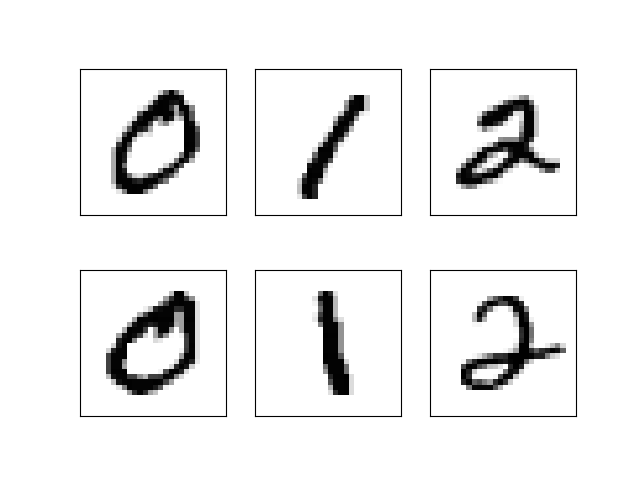
\includegraphics[scale=0.3]{images/mnist_experiment/mnist_digits.png}
  \caption{Example inputs from MNIST data set. The models are trained on zeros and ones (in-distribution), then shown varying quantities of twos (out-of-distribution) at test time.}
  \label{mnist_inputs_image}
\end{figure}

\begin{figure}
  \centering
  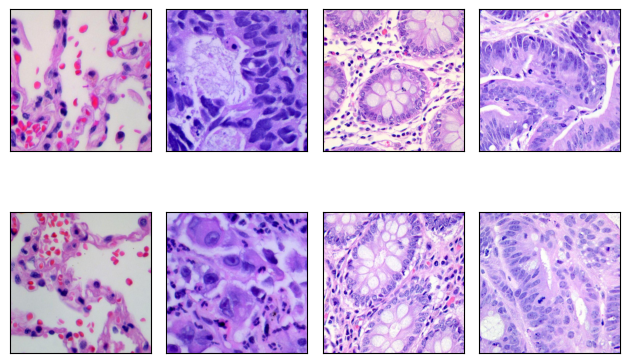
\includegraphics[scale=0.5]{images/cancer_experiment/cancer_images.png}
  \caption{Example inputs from lung and colon tissue data set. Left to right: Benign lung, cancerous lung, benign colon, cancerous colon. The models are trained on lung images (in-distribution), then shown varying quantities of colon images (out-of-distribution) at test time.}
  \label{cancer_inputs_image}
\end{figure}



\section{Distance measures}
\label{sec:distance measures}
It is instructive to study the latent space of a simple model to gain an intuition of what this reveals of the model's behaviour. The CNN trained in Section \ref{sec:mnist method} contains two neurons in its final hidden layer, so the positions of points can be visualised in 2D latent space. This is used to guide the design of distance measures in this section.

\subsection{Interpreting the latent space}
\label{sec:interpret latent space}

The positions of zeros and ones (in-distribution) and twos (out-of-distribution) in the 2-dimensional latent space of the CNN model are shown in Figure \ref{latents_2d}. The model learns to separate the in-distribution samples; zeros are aligned with the x-axis and ones with the y-axis. This is consistent with the interpretation of a  neural network trained for binary classification as a kernel logistic regression model, where the hidden layers effectively learn a non-linear kernel to separate the classes in latent space, and the final softmax layer is a typical logistic regression \cite{pmlr-v202-guyomard23a}.

In contrast, the out-of-distribution data, i.e. the twos, lie in the middle of the latent space suggesting that the model is less able to distinguish these from the ones. Of note here is that they do generally lie closer to the cluster of zeros (the negative classification) than the cluster of ones (the positive classification). This is the correct classification for our model trained to identify ones, which implies that we may still get reasonable accuracy in practice despite having never seen similar data before, therefore relying on accuracy metrics alone could be instil a misplaced sense of confidence in the model's appropriateness; the \emph{confidence} in this model should be lower in this scenario even if the predictions are correct.

The effect of applying Simplex to this data is shown in Figure \ref{residual_shift_2d}. The in-distribution samples are shifted along their respective axes towards the centre of the cluster of that digit. This is consistent with the idea behind Simplex that "outlier" points are approximated by a combination of points in the corpus hull. In contrast, the out-of-distribution digits do not move in a consistent direction, reflecting that the model is unable to reconstruct them consistently using the corpus, but that the basis vectors provided by the corpus span the required latent space. This can be observed in Figure \ref{residuals_2d} which shows the residual vectors in latent space.

The same approach is repeated for the 3-dimensional case to verify that similar relations hold using a new CNN is created with 3 neurons in its last hidden layer. Following the same approach, in Figure \ref{latents_3d} the in-distribution data points again form linearly separable clusters in 3D latent space, while the out-of-distribution data lies in between. In Figures \ref{residual_shift_3d} and \ref{residuals_3d}, it is again observed that the Simplex approximations bring points closer towards the centre of clusters.
\footnote{Interactive versions of these 3D plots illustrate this more clearly. These are available in the Github repository for the
\href{https://htmlpreview.github.io/?https://github.com/gjohl/xai/blob/master/xai/experiments/report_figures/latent_space/interactive_latent_space_scatter_3d.html}{latent space distribution}
, the
\href{https://htmlpreview.github.io/?https://github.com/gjohl/xai/blob/master/xai/experiments/report_figures/latent_space/interactive_residuals_3d.html}{residual distribution}
and an
\href{https://htmlpreview.github.io/?https://github.com/gjohl/xai/blob/master/xai/experiments/report_figures/latent_space/interactive_residual_shift_3d.html}{interactive time lapse animation of the residual shift.}
}


% TODO GJ: Figure formatting
\begin{figure}[h]
\centering
\begin{minipage}{.25\textwidth}
  \centering
  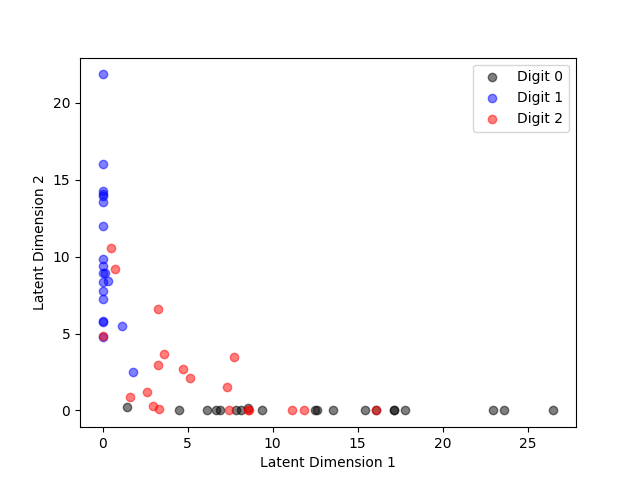
\includegraphics[width=.8\linewidth]{images/latent_space/latent_space_scatter_2d.png}
  \captionof{figure}{Distribution of a sample of digits in the model's latent space.}
  \label{latents_2d}
\end{minipage}%
\hspace{.05\textwidth}
\begin{minipage}{.25\textwidth}
  \centering
  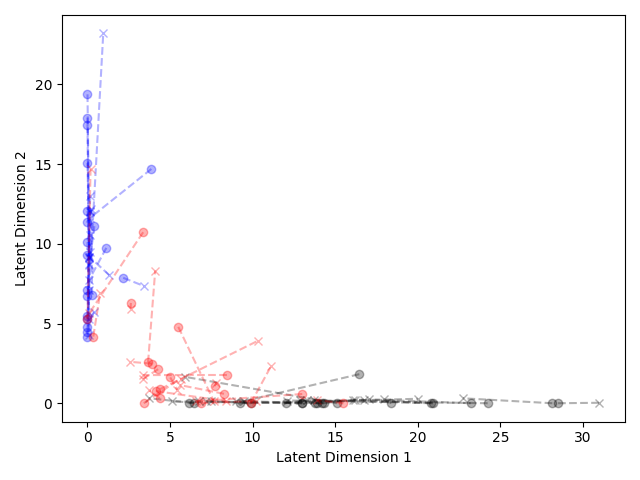
\includegraphics[width=.8\linewidth]{images/latent_space/residual_shift_2d.png}
  \captionof{figure}
  {Residual shift of true values (circles) to their Simplex approximation (crosses).}
  \label{residual_shift_2d}
\end{minipage}
\begin{minipage}{.25\textwidth}
  \centering
  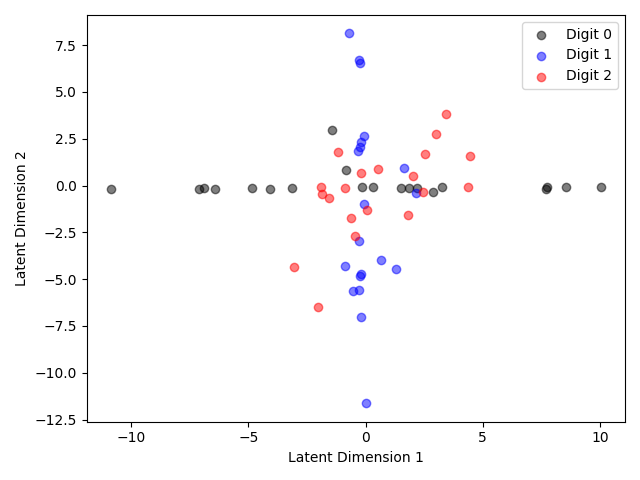
\includegraphics[width=.8\linewidth]{images/latent_space/residuals_2d.png}
  \captionof{figure}
  {Residual vectors in the model's latent space.}
  \label{residuals_2d}
\end{minipage}
\end{figure}


\begin{figure}[h]
\centering
\begin{minipage}{.25\textwidth}
  \centering
  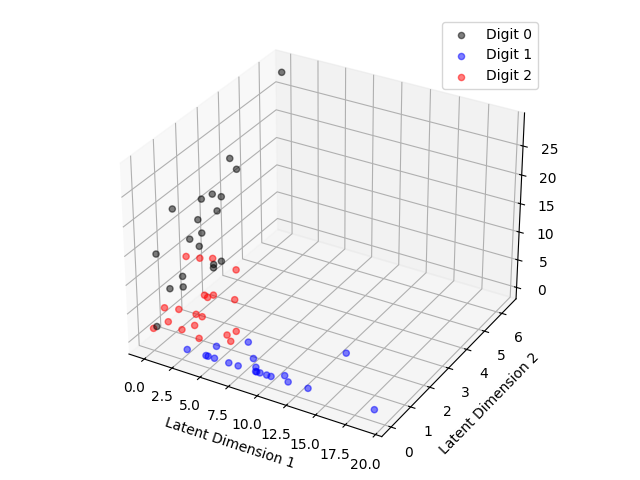
\includegraphics[width=.8\linewidth]{images/latent_space/latent_space_scatter_3d.png}
  \captionof{figure}{Distribution of a sample of digits in the model's latent space.}
  \label{latents_3d}
\end{minipage}%
\hspace{.05\textwidth}
\begin{minipage}{.25\textwidth}
  \centering
  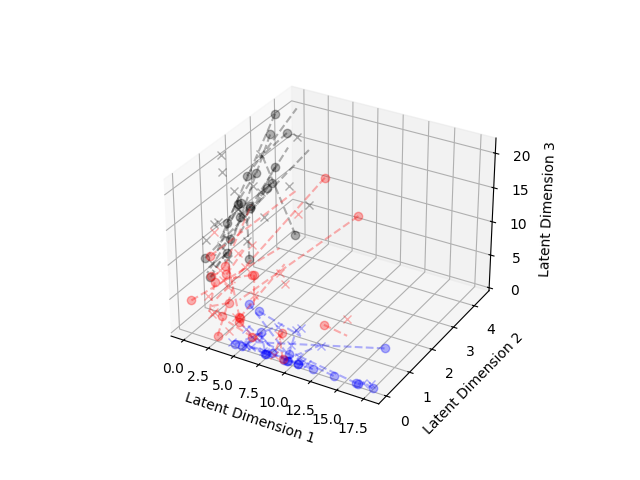
\includegraphics[width=.8\linewidth]{images/latent_space/residual_shift_3d.png}
  \captionof{figure}
  {Residual shift of true values (circles) to their Simplex approximation (crosses).}
  \label{residual_shift_3d}
\end{minipage}
\begin{minipage}{.25\textwidth}
  \centering
  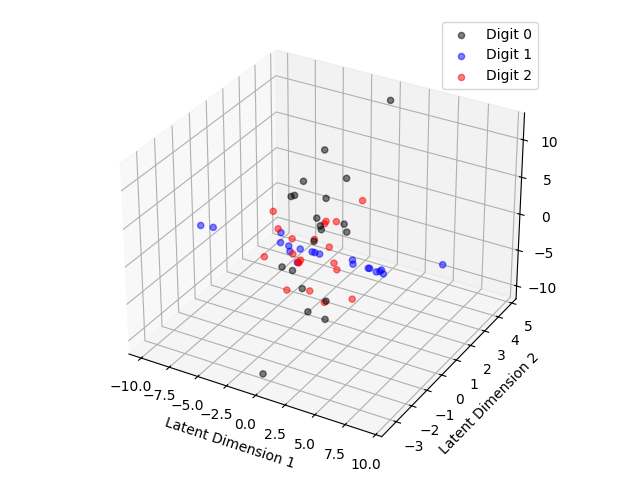
\includegraphics[width=.8\linewidth]{images/latent_space/residuals_3d.png}
  \captionof{figure}
  {Residual vectors in the model's latent space.}
  \label{residuals_3d}
\end{minipage}
\end{figure}


\subsection{Distance measures formulations}
\label{sec:distance measures}
A set of distance measures is proposed in this section, guided by the experimental insights above. These are then applied to the two data sets in Section \ref{sec:results section} to establish their relation to the OOD proportion, i.e. the level of extrapolation.

A natural starting point for a distance measure is to use the residual vectors of the Simplex approximation, which measure of how closely a test example can be decomposed as a combination of corpus inputs. This is the motivation behind the $r_norm$ distance measure, which calculates the vector norm of each residual example, and averages this over the test data set.
\begin{equation}
\label{eq:r norm}
	r_{norm} = \frac{\sum_i^n ||\bm{r_{test_i}}||_2}{n}  \forall i  \in \bm{D_{test}}
\end{equation}

One may initially expect this to be larger for OOD data points, but as observed in Figures \ref{residual_shift_2d} and \ref{residuals_2d}, the in-distribution points move along the axis, whereas OOD points move more randomly and begin closer to the centre of the latent space, so their residuals are actually smaller. This direction-specific movement is of particular interest, and forms the basis of later distance measures.

The next straightforward measure is to take the norm of the latent space. As observed in Figure \ref{latents_2d} and \ref{latents_3d}, the in-distribution points are separated by the classifier, whereas OOD points cluster towards the centre of the latent space. Therefore, this should provide some some measure of the shrinkage of the latent space
\begin{equation}
\label{eq:h norm}
	h_{norm} = ||\bm{H_{test}}||_2
\end{equation}

A variation of this approach is introduced to address the fact that if one class has OOD points but the other does not (as in the MNIST experiment where we have OOD negative classifications but not positive classifications) then the latent space occupied by each predicted classification may shrink at different rates. If the number of samples in each class was imbalanced, this observation could contain useful information. The next measure separates points by their predicted classification before calculating the norm of each, then returns the weighted average of class-wise norms.
\begin{equation}
\label{eq:h norm classwise}
	h_{norm\_classwise} =\sum_c \frac{|\bm{D_{test_{\hat{y}=c}}}|}{|\bm{D_{test}}|} \cdot ||\bm{H_{test_{\hat{y}=c}}}||_2 \forall c \in  [0, 1]
\end{equation}

A direction-wise variant of this measure, $h_{norm\_directionwise}$, is calculated, noting that the in-distribution points of a given class generally occupy a particular hyperplane of the latent space, so the out-of-plane axis for the true class is generally noise. We expect this noise to be higher for OOD points than in-distribution points. The out-of-plane axis is determined by selecting the axis with the smallest standard deviation for the validation set. The calculation is then identical to Equation \ref{eq:h norm classwise}.

Relative variants of each of the above measures are obtained by taking the ratio of $h_{norm}$ values between the test set and the latent approximation of the validation set under Simplex. Using a validation set in this way resembles the calibration set used for the deep k-nearest neighbours approach \cite{papernot_deep_2018}. This allows for more interpretable scales---a value of 1 for $h_{rel\_norm}$ or $h_{rel\_norm\_classwise}$ indicates that the test set came from a similar distribution as the in-distribution validation set, whereas a smaller value suggests the test contains more OOD data, which shrinks the latent space towards the centre. For $h_{rel\_norm\_directionwise}$ the value should increase with OOD data as these are typically further out-of-plane.
\begin{equation}
\label{eq:relative h norm}
	h_{rel\_norm} = \frac{h_{norm_{test}}}{\hat{h}_{norm_{validation}}}
\end{equation}



\section{Results}
\label{sec:results section}
The results of the proposed experiments are provided here, firstly for handwritten digit data in Section \ref{sec:mnist results} and then to a real data set of histopathological images in Section \ref{sec:cancer results}.


\subsection{MNIST classification experiment results}
\label{sec:mnist results}
As a benchmark, common performance metrics accuracy and AUC are shown in Figure \ref{res:mnist accuracy}, as well as the the mean of the probabilities output by the model which are commonly cited as a measure of confidence. It is observed that accuracy and AUC both decrease as the OOD proportion increases, which is expected, though their absolute values are still relatively high; a practitioner may well still choose such a model on the basis of these values, not knowing that their data set is so far removed from the model's training data.
The model probabilities are high across all levels of OOD, corroborating the observations of Papernot and McDaniel in the context of Deep kNN that model probabilities are poor proxies of confidence, despite being widely used for this purpose \cite{papernot_deep_2018}. The dispersion of probabilities does show some relation to the OOD proportion, shown in Figure \ref{res:mnist prob std}.

The values of $h_{norm}$ and $h_{norm\_classwise}$ are shown in Figure \ref{res:mnist h norm}, a residual-based measure $r_{norm}$ in Figure \ref{res:mnist r norm}, and relative distance measures $h_{rel\_norm}$ and $h_{rel\_norm\_classwise}$ in Figure \ref{res:mnist relative h norm}.
These all decrease as OOD points are added, in line with the understanding that OOD points lie in the middle of the space whereas in-distribution points a separated to the extremes. Also observed is similarity between  $h_{rel\_norm}$ and $h_{rel\_norm\_classwise}$, owing to the balanced classes of the experimental design. The behaviour in cases of imbalanced classes is a topic of further research.

The direction-specific relative measure $h_{rel\_norm\_directionwise}$, which isolates the out-of-plane axis, is shown in Figure \ref{res:mnist relative h norm directionwise}.
This increases with OOD because in-distribution points typically lie in the plane whereas OOD points are more scattered.


\begin{figure}[h]
\centering
\begin{minipage}{.25\textwidth}
  \centering
  \includegraphics[width=.8\linewidth]{images/mnist_experiment/classification_metrics.png}
  \captionof{figure}{Classification metrics for MNIST data.}
  \label{res:mnist accuracy}
\end{minipage}%
\hspace{.05\textwidth}
\begin{minipage}{.25\textwidth}
  \centering
  \includegraphics[width=.8\linewidth]{images/mnist_experiment/probability_std_dev.png}
  \captionof{figure}
  {Standard deviation of model probabilities.}
  \label{res:mnist prob std}
\end{minipage}
\begin{minipage}{.25\textwidth}
  \centering
  \includegraphics[width=.8\linewidth]{images/mnist_experiment/h_norm.png}
  \captionof{figure}
  {Norm of latent space.}
  \label{res:mnist h norm}
\end{minipage}
\end{figure}


\begin{figure}[h]
\centering
\begin{minipage}{.25\textwidth}
  \centering
  \includegraphics[width=.8\linewidth]{images/mnist_experiment/residual_norm.png}
  \captionof{figure}{Norm of residuals.}
  \label{res:mnist r norm}
\end{minipage}%
\hspace{.05\textwidth}
\begin{minipage}{.25\textwidth}
  \centering
  \includegraphics[width=.8\linewidth]{images/mnist_experiment/relative_h_norm.png}
  \captionof{figure}{Ratio of test and validation latent space norms.}
  \label{res:mnist relative h norm}
\end{minipage}
\begin{minipage}{.25\textwidth}
  \centering
  \includegraphics[width=.8\linewidth]{images/mnist_experiment/relative_h_norm_directionwise.png}
  \captionof{figure}{Ratio of test and validation latent space norms in the out-of-plane axis.}
  \label{res:mnist relative h norm directionwise}
\end{minipage}
\end{figure}





\subsection{Cancer classification experiment results}
\label{sec:cancer results}
The results for a similar experiment on the tissue image data set shows largely consistent results, see Figures \ref{res:cancer accuracy} to \ref{res:cancer relative h norm directionwise}. This is encouraging, as it suggests that the conclusions drawn about Simplex-based confidence measures generalise to real-world data sets, and may therefore be useful to aid practitioners in understanding and applying models.

The only notable difference is the behaviour of the direction-specific latent space norm in Figure \ref{res:cancer relative h norm directionwise}. This may be due to the different dimensionality of the latent space of the model used for this experiment. For each class in the data, this measure isolates the dimension with the smallest variance in the validation data as the noise axis. This approach worked for the MNIST model with 2D latent space. For higher dimensions, this may not be as appropriate if the IDD points lie in a plane that is not aligned with the axes. An alternative methodology may be more robust in higher dimensions, where the covariance matrix of each class in the validation set is used to identify a variable number of axes to isolate. This is an area of further research.



\begin{figure}[h]
\centering
\begin{minipage}{.25\textwidth}
  \centering
  \includegraphics[width=.8\linewidth]{images/cancer_experiment/classification_metrics.png}
  \captionof{figure}{Classification metrics for tissue images.}
  \label{res:cancer accuracy}
\end{minipage}%
\hspace{.05\textwidth}
\begin{minipage}{.25\textwidth}
  \centering
  \includegraphics[width=.8\linewidth]{images/cancer_experiment/probability_std_dev.png}
  \captionof{figure}
  {Standard deviation of model probabilities.}
  \label{res:cancer prob std}
\end{minipage}
\begin{minipage}{.25\textwidth}
  \centering
  \includegraphics[width=.8\linewidth]{images/cancer_experiment/h_norm.png}
  \captionof{figure}
  {Norm of latent space.}
  \label{res:cancer h norm}
\end{minipage}
\end{figure}


\begin{figure}[h]
\centering
\begin{minipage}{.25\textwidth}
  \centering
  \includegraphics[width=.8\linewidth]{images/cancer_experiment/residual_norm.png}
  \captionof{figure}{Norm of residuals.}
  \label{res:cancer r norm}
\end{minipage}%
\hspace{.05\textwidth}
\begin{minipage}{.25\textwidth}
  \centering
  \includegraphics[width=.8\linewidth]{images/cancer_experiment/relative_h_norm.png}
  \captionof{figure}{Ratio of test and validation latent space norms}
  \label{res:cancer relative h norm}
\end{minipage}
\begin{minipage}{.25\textwidth}
  \centering
  \includegraphics[width=.8\linewidth]{images/cancer_experiment/relative_h_norm_directionwise.png}
  \captionof{figure}{Ratio of test and validation latent space norms in the out-of-plane axis.}
  \label{res:cancer relative h norm directionwise}
\end{minipage}
\end{figure}



\section{Conclusions}

The Simplex approach to the latent space and its approximations was used to form several distance measures that can act as a measure of confidence in the model for the given application.
An intuitive understanding of the latent space of a model was explored by examining simple models in 2D and 3D for in-distribution and out-of-distribution data.
This helps to understand the behaviour of a model, which in turn guided the formulation of distance metrics. These provide a global quantification of extrapolation which can serve as a confidence measure.

These distance measures were applied to two binary classification tasks in an experimental setup that allowed us to vary the ground truth level of extrapolation.
In both experiments, we show that the distance measures correspond with the level of extrapolation by varying the degree of out-of-distribution samples in the test set.
This can be used to supplement accuracy measurements to guide practitioners when selecting a model and understanding when a model is operating beyond its intended use case.

Armed with this knowledge, the practitioner can either select a more appropriate model or address the cause of extrapolation, which can be done using the original Simplex method to understand individual instances either in terms of their features or corpus examples. This can identify aleatoric uncertainty caused by missing features or biases causes by underrepresented examples in the training data, both of which can exacerbate healthcare inequity. Thus, this approach could be a useful approach in the burgeoning field of data-centric AI \cite{zha_data-centric_2023}.

The consequence of the extension proposed in this work is that the Simplex approach can be applied top-down to the data set at a high-level, and then used to investigate further on the basis of features or examples, providing a holistic solution to understanding the interaction between data and models.



\section{Future work}
\label{sec:future work}

The approach of using latent space representations and approximations as a measure of confidence can be extended further across different distance formulations, tasks and domains, as well as linking with the related areas of model design, transfer learning and data-centric AI.

% From https://miro.com/welcomeonboard/M3RaRnphQWFISWx0V3dJeVhhNGNrd3MwQXdRTXgxeGlWM1J2TTQ5RHpFb21lb2M1VEQxU211bDRaa1F0dVRGVHwzMDc0NDU3MzQ4NjkzNjkyODM1fDI=?share_link_id=231878117892
\begin{figure}[ht]
  \centering
  % \fbox{\rule[-.5cm]{0cm}{4cm} \rule[-.5cm]{4cm}{0cm}}
  \includegraphics[scale=0.07]{images/explainability_feedback_loop.jpg}
  \caption{Using explainability methods to continuously improve models and data. The solid black arrows show the flow of data in current paradigms, where a model generates outputs from data and a post-hoc explainer can interpret the model's behaviour. The dashed lines show how global explainability measures can facilitate a feedback loop where models and data can be improved based on the explainer.}
  \label{explainability_loop}
\end{figure}


\paragraph{Variations and comparisons with other distance measures}
Alternative formulations of distance measures based on latent spaces and Simplex approximations could be explored, some of which were noted in discussion of results.
Calibrating these measures experimentally on different models and data sets, as well as theoretical guarantees for such measures, are areas of further research.
The effectiveness of using validation sets from data sets other than that used to train the model could be investigated. This would allow the approach to be used in cases where the training data is not available, for example, where privacy concerns limit dissemination of the training data.
The approach could also be applied over multiple hidden layers of the model and aggregated, as in the Deep KNN approach, rather than using only the final hidden layers. The measures here could be benchmarked against other approaches, including Deep KNN, as well as more traditional measures of distance used in transfer learning \cite{zhuang_comprehensive_2021}, such as KL-divergence and Maximum Mean Discrepancy, both in the input space and latent space.
% Approximate distances based on centroid for faster computation. Cite need for faster computation. Day and Khoshgoftaar, Page 38: “there is a need to investigate and develop highly computationally efficient methods which can be applied to large datasets.” \cite{day_survey_2017}

\paragraph{Additional tasks and domains}
The experiments here only considered the task of binary classification. Further work could explore the latent space for other supervised tasks---multiclass classification, regression---as well as unsupervised tasks.
The experiments in this paper used image data, owing to the availability of public image data sets and well-established performance of CNNs on these tasks. None of the concepts discussed are specific to computer vision, so further work could explore other domains such as text data, tabular data and time series data which is particularly pertinent in healthcare settings.

\paragraph{Transfer learning} \label{sec:transfer learning}
Transfer learning is an increasingly important topic with the proliferation of pre-trained foundational models.
This has implications in healthcare, where the application of such models could provide powerful predictions on small data sets, provided the user can evaluate the confidence of the model. This could allow for more powerful individualised models, where a foundational model can be trained on the health records of a particular patient or group of patients.
A method of measuring the transferability of a model across domains is an open question \cite{pan_survey_2010} \cite{zhuang_comprehensive_2021}. The intuitive requirements for such a measure are that it be a model-specific measure between  a source data set $D_{source}$ and target data set $D_{target}$. This therefore bears a close resemblance to \ref{general_confidence_form}.
The open question of identifying and explaining negative transfer could also be explored by researching behaviour in the latent space.
A related research area noted by \cite{zhuang_comprehensive_2021} is \emph{interpretability} of transfer. The approach explored in this paper is rooted in explainability methods and therefore naturally addresses this concern.

\paragraph{Model design}
With appropriate scaling of the distance measures proposed in this paper, we can compare confidence between different models to answer the question of which model best explains a given data set. Where no satisfactory models are found, this can influence the design of model architecture to better capture the unexplained information.


\paragraph{Data-centric AI}
The approach outlined here can be used to identify data sets which are poorly described by existing models, i.e. where substantial extrapolation is required.
These can be explored in-depth by explaining the poorly approximated test data in terms of features or examples, as in the original paper \cite{crabbe_explaining_2021}.
The feature-based approach can identify cases where features are not informative enough and may benefit from collecting additional fields.
The example-based approach can identify cases where particular test instances are underrepresented in the test data, for example when specific ethnic groups are not represented in the training data and therefore would be at risk of misclassification by the model.
This could also identify areas of the latent space where synthetic data could be utilised.
Identifying these biases and having the tools to address them can play an important role in improving input data and addressing healthcare inequity.

\paragraph{Continuous improvement of model and data}
Taking the above two points of model design and data improvement in tandem suggests an iterative approach to applying machine learning models, whereby explanations of the model on a data set reveal shortcomings of both model and data, which can each in turn be addressed and revised.
By linking explainability with model design and data collection, it can be framed as a key component in performance and ultimately healthcare outcomes. Not only does better explainability aid human understanding, it can be employed as a tactic in improving the models themselves and addressing biases in data, leading to improved outcomes.



% To make sure figures display before references
\clearpage

\bibliographystyle{unsrt}
\bibliography{references}


% -------------------UNUSED--------------------------
% This section is just for commands from the original template that might be useful for reference

% \section{Useful commands}
% \url{https://neurips.cc/public/guides/PaperChecklist}. \\
% {\bf nine} \\
% \emph{containing only acknowledgments and references} \\
% \nicefrac{1}{2}
% \begin{center}
%   \url{http://www.neurips.cc/}
% \end{center} \\
% \verb+final+  \\
% Of note is the command \verb+\citet+, which produces citations appropriate for
% use in inline text.  For example,
% \begin{verbatim}
%    \citet{hasselmo} investigated\dots
% \end{verbatim}
% produces
% \begin{quote}
%   Hasselmo, et al.\ (1995) investigated\dots
% \end{quote}

% The formatting instructions contained in these style files are summarized in
% Sections \ref{headings} below.




% \section{Headings: first level}
% \label{headings}


% All headings should be lower case (except for first word and proper nouns),
% flush left, and bold.


% First-level headings should be in 12-point type.


% \subsection{Headings: second level}


% Second-level headings should be in 10-point type.


% \subsubsection{Headings: third level}


% Third-level headings should be in 10-point type.


% \paragraph{Paragraphs}


% There is also a \verb+\paragraph+ command available, which sets the heading in
% bold, flush left, and inline with the text, with the heading followed by 1\,em
% of space.



% \subsection{Footnotes}

% Indicate footnotes with a number\footnote{Sample of the first footnote.} in the
% text. Place the footnotes at the bottom of the page on which they appear.

% Note that footnotes are properly typeset \emph{after} punctuation
% marks.\footnote{As in this example.}


% \subsection{Figures}


% \begin{figure}
%   \centering
%   \fbox{\rule[-.5cm]{0cm}{4cm} \rule[-.5cm]{4cm}{0cm}}
%   \caption{Sample figure caption.}
% \end{figure}

% The figure caption should be lower case (except for first word and
% proper nouns); figures are numbered consecutively.


% \subsection{Tables}

% All tables must be centered, neat, clean and legible.  The table number and
% title always appear before the table.  See Table~\ref{sample-table}.


% The table title must be lower case (except for first word and proper nouns); tables are numbered consecutively.


% Note that publication-quality tables \emph{do not contain vertical rules.} We
% strongly suggest the use of the \verb+booktabs+ package, which allows for
% typesetting high-quality, professional tables:
% \begin{center}
%   \url{https://www.ctan.org/pkg/booktabs}
% \end{center}
% This package was used to typeset Table~\ref{sample-table}.


% \begin{table}
%   \caption{Sample table title}
%   \label{sample-table}
%   \centering
%   \begin{tabular}{lll}
%     \toprule
%     \multicolumn{2}{c}{Part}                   \\
%     \cmidrule(r){1-2}
%     Name     & Description     & Size ($\mu$m) \\
%     \midrule
%     Dendrite & Input terminal  & $\sim$100     \\
%     Axon     & Output terminal & $\sim$10      \\
%     Soma     & Cell body       & up to $10^6$  \\
%     \bottomrule
%   \end{tabular}
% \end{table}

% \subsection{Math}
% Note that display math in bare TeX commands will not create correct line numbers for submission. Please use LaTeX (or AMSTeX) commands for unnumbered display math. (You really shouldn't be using \$\$ anyway; see \url{https://tex.stackexchange.com/questions/503/why-is-preferable-to} and \url{https://tex.stackexchange.com/questions/40492/what-are-the-differences-between-align-equation-and-displaymath} for more information.)


% \section{Preparing PDF files}


% Please prepare submission files with paper size ``US Letter,'' and not, for
% example, ``A4.''


% \subsection{Margins in \LaTeX{}}

% Most of the margin problems come from figures positioned by hand using
% \verb+\special+ or other commands. We suggest using the command
% \verb+\includegraphics+ from the \verb+graphicx+ package. Always specify the
% figure width as a multiple of the line width as in the example below:
% \begin{verbatim}
%    \usepackage[pdftex]{graphicx} ...
%    \includegraphics[width=0.8\linewidth]{myfile.pdf}
% \end{verbatim}
% See Section 4.4 in the graphics bundle documentation
% (\url{http://mirrors.ctan.org/macros/latex/required/graphics/grfguide.pdf})


% \begin{ack}
% Use unnumbered first level headings for the acknowledgments. All acknowledgments
% go at the end of the paper before the list of references.
% \end{ack}


% \section*{References}

% \medskip


% {
% \small


% [1] Alexander, J.A.\ \& Mozer, M.C.\ (1995) Template-based algorithms for
% connectionist rule extraction. In G.\ Tesauro, D.S.\ Touretzky and T.K.\ Leen
% (eds.), {\it Advances in Neural Information Processing Systems 7},
% pp.\ 609--616. Cambridge, MA: MIT Press.


% [2] Bower, J.M.\ \& Beeman, D.\ (1995) {\it The Book of GENESIS: Exploring
%   Realistic Neural Models with the GEneral NEural SImulation System.}  New York:
% TELOS/Springer--Verlag.


% [3] Hasselmo, M.E., Schnell, E.\ \& Barkai, E.\ (1995) Dynamics of learning and
% recall at excitatory recurrent synapses and cholinergic modulation in rat
% hippocampal region CA3. {\it Journal of Neuroscience} {\bf 15}(7):5249-5262.
% }

% %%%%%%%%%%%%%%%%%%%%%%%%%%%%%%%%%%%%%%%%%%%%%%%%%%%%%%%%%%%%


\end{document}